\documentclass{article}

\usepackage{fancyhdr} % Required for custom headers
\usepackage[utf8]{inputenc}
\usepackage{lastpage} % Required to determine the last page for the footer
\usepackage{extramarks} % Required for headers and footers
\usepackage[usenames,dvipsnames]{color} % Required for custom colors
\usepackage{graphicx} % Required to insert images
\usepackage{listings} % Required for insertion of code
\usepackage{courier} % Required for the courier font
\usepackage{lipsum} % Used for inserting dummy 'Lorem ipsum' text into the template
\usepackage{lstlangarm}

% Margins
\topmargin=-0.45in
\evensidemargin=0in
\oddsidemargin=0in
\textwidth=6.5in
\textheight=9.0in
\headsep=0.25in

\linespread{1.1} % Line spacing

% Set up the header and footer
\pagestyle{fancy}

\lhead{\exerciseGroup} % Top left header
\chead{\exerciseClass: \exerciseTitle} % Top center head
\rhead{\firstxmark} % Top right header
\lfoot{\lastxmark} % Bottom left footer
\cfoot{} % Bottom center footer
\rfoot{Page\ \thepage\ of\ \protect\pageref{LastPage}} % Bottom right footer
\renewcommand\headrulewidth{0.4pt} % Size of the header rule
\renewcommand\footrulewidth{0.4pt} % Size of the footer rule

\setlength\parindent{0pt} % Removes all indentation from paragraphs


% Document data

\newcommand{\exerciseTitle}{Exericse 1} % Assignment title
\newcommand{\exerciseClass}{TDT4258} % Course/class
\newcommand{\exerciseGroup}{Group 1} % Your name
\newcommand{\exerciseGroupMembers}{Kim Rune Solstad, Sindre Magnussen and Håkon Åmdal}
\newcommand{\chipName}{EFM32 Giant Gecko}
%----------------------------------------------------------------------------------------
%	TITLE PAGE
%----------------------------------------------------------------------------------------

\title{
\vspace{2in}
\textmd{\textbf{\exerciseClass: \exerciseTitle}}\\
\vspace{3in}
\exerciseGroupMembers
}

\author{\textbf{\exerciseGroup}}
\date{} % Insert date here if you want it to appear below your name

%----------------------------------------------------------------------------------------

% -------
% Bibliography
% -------



\begin{document}

\maketitle

\newpage \begin{abstract}
\end{abstract}


\newpage \tableofcontents

\newpage \section{Introduction}
In this exercise, we were supposed to implement a system that let the user control the LEDs in some way by pressing the gamepad buttons. We were also required to implement the functionality by using an interrupt routine. During the solving of this task, we were supposed to analyze the power consumption and correctness of the system. The learning outcome of this task was (as stated in \cite[p. 19]{compendium}):
\begin{itemize}
	\item Get to know the \boardName, the GPIO and the ARM Cortex-M3 arcitechture.
	\item Get to know the GNU toolchain, object files and the task of a linker.
	\item Programming in assembly for the ARM Cortex-M3.
	\item Measuring and optimizing power consumption.
\end{itemize}
We approached the task by first creating a simple program which we graudually improved the energy efficiency of by intrudocing interrupts and various operational modes. Then we implemented a more advanced program to practise our assembly skills and see if added functionality required us to change operational mode. During the development we tested for correctness and power consumption continiously, which maximized the learning outcome of this task.



\newpage \section{Description and Methodology}

\subsection{Compiling the Linux kernel}
\begin{figure}[h]
	\centering
	
\includegraphics[width=3cm]{img/uclinux.png}
	\caption{uClinux logo}
	\label{fig:uclinux}
\end{figure}
We were supplied with a variant of Linux called \emph{uClinux}, and it's supplied toolchain. We built the distribution by using a build system named \emph{ptxdist}. We followed \cite[section 5.3]{compendium} step by step, and when done we ended up with a working linux distribuion on the chip, with Tux drawn on the screen. Initially we did not change the kernel config\footnote{We ended up doing so, please see section \ref{subsection:energy-efficiency}.}, nor add any more packages than already supplied and configured.

\subsection{Device driver for the gamepad}

\subsubsection{Linux kernel module}
Oppsett\\
Opprydding
\subsubsection{Linux character driver}
Oppsett\\
opprydding
\subsubsection{Character device operations}

\paragraph{Open}
\paragraph{Clone}
\paragraph{Read}
\paragraph{Write}

\subsection{Signals and interrupts}
\label{subsection:signals-and-interrupts}
Based on previous experience regarding energy efficiency, we decided to implement our driver with interrupts and signals right away.
\subsubsection{Enabling and handling interrupts}

Enabling interrupt is done in the \emph{tdt4258\_gamepad\_probe()} method, in the same fashion as the two previous exercises. The only difference is that we write to the specific registers using \emph{iowrite32()} to make the code more portable for virtual memory. For more information about enabling interrupts for the GPIO-controller, see \cite[section 3]{compendium}. We also have to save the IRQ-numbers for the GPIO, for later use. This is done by calling \emph{platform\_get\_irq()} on the platform device that is passed as parameter to the probe function.\\

When a user application calls \emph{open()}, we register the method \emph{gpio\_interrupt\_handler()} as the interrupt handler for the odd and even GPIO PC pins. This is done using the system call \emph{request\_irq()}\footnote{http://www.makelinux.net/books/lkd2/ch06lev1sec3}. The GPIO-handler simply reads and saves the button value and signals the user application that the buttons value has changed. It is also responsible of clearing the interrupt (see \cite[section 3]{compendium} and the code).   

\subsubsection{Generating signals in kernel space}
\begin{figure}[h]
	\centering
	\lstinputlisting[frame=single, numbers=left]{code/signal_user_application.c}
	\caption{Signaling user space from kernel space}
	\label{fig:signal-user-application}
\end{figure}
The \vn{signal\_user\_application(void)} function in the \mn{driver-gamepad.c} sends a signal to the process who has the driver open. We have used the \textbf{SIGUSR1} signal, because it is documented to be set aside for you to use any way we want and is useful for interprocess communication. In addition to specifying signal type and process to receive the signal, we add the SI\_QUEUE to enable the signal to carry data from kernel to user space. See figure \ref{fig:signal-user-application}.

\subsection{The game application}
Here is a little overview of the files in the game application. There will not be a thorough explanation of the code, as it is well documented.

\begin{itemize}
	\item \mn{game.c} - Main game module. Will initialize signal handlers and external modules, register button and timer handlers and start a \vn{pause()} loop. 
	\item \mn{input.c} - Handles gamepad input. Contains the driver file handle and a list of button handlers. It will determine which button(s) is pressed and/or released, and call the corresponding handlers.
	\item \mn{pong.c} - This module contains all logic for the Pong game. A more detailed explanation is found in section \ref{subsection:pong}.
	\item \mn{screen.c} - This module handles the screen driver file handle, and takes care of drawing and updating the frame buffer device.
	\item \mn{signal.c} - Module that enables signal handlers for \textbf{SIGALRM} and \textbf{SIGUSR1}.
	\item \mn{timer.c} - This module will set up the timer with a given interval, and keep track of which function that should be called on each timer tick. This is needed to animate the game.
\end{itemize}

Most of the C source files have a corresponding header to define their external interfaces.

\subsubsection{The pause() loop}
\begin{figure}[h]
	\centering
	\lstinputlisting[frame=single, numbers=left]{code/pause_loop.c}
	\caption{The pause loop}
	\label{fig:pause-loop}
\end{figure}
The main program will live in a \vn{pause()}\footnote{http://linux.die.net/man/2/pause} loop during execution. This function sleeps until a signal is delivered.

\subsubsection{Timer}
\begin{figure}[h]
	\centering
	\lstinputlisting[frame=single, numbers=left]{code/setitimer.c}
	\caption{Starting the system timer}
	\label{fig:setitimer}
\end{figure}
The \mn{timer.c} module will start a system timer, using the \vn{setitimer()}\footnote{http://linux.die.net/man/2/setitimer} procedure defined in the C standard library (se figure \ref{fig:setitimer}). On each timer tick, the \textbf{SIGALRM} signal will be sent to the process, which is handeled in \mn{signal.c} and delegated back to \mn{timer.c}.

\subsubsection{Handling signals in user space}
\begin{figure}[h]
	\centering
	\lstinputlisting[frame=single, numbers=left]{code/sighandler.c}
	\caption{Adding signals handlers with signal mask to the user space}
	\label{fig:sighandler}
\end{figure}
We needed to configure our application \textbf{SIGUSR1} and \textbf{SIGALRM} signals. See figure \ref{fig:sighandler}. The handlers called respective methods in \mn{timer.c} and \mn{input.c}.\\
\\
In other words, with the main program spinning in the \vn{pause()} loop, all of the program work is done entirely by the signal handlers.


\subsection{Controlling the framebuffer device}
The EFM32GG has it's own framebuffer device that manages the display. This device is accessed by opening the driver \emph{/dev/fb0} as a file. When the file is opened, we have access to the drivers methods. As described in \cite[section 5.4.2]{compendium}, this means that we can use \emph{read()}, \emph{write()} and \emph{lseek()} wich can be used to handle the frambuffer byte by byte as a usual file. But, as \cite[section 5.4.2]{compendium} describes, there is a way controlling the frambuffer that is easier and faster then using the mentioned method. \\

The framebuffer device can be memory mapped. This means that we can map the driver to an array in memory, which in C means that we are able to write pixels directly with an usual C array. This done by calling the function \emph{mmap()}, wich is a Unix system call declared in the header \emph{sys/mmap.h}. 
Writing to the array will update a buffer holding the pixel values. To write the changes in the framebuffer to the display we use the system call \emph{ioctl()}. \\

\emph{ioctl()} is driver specific system call, and can be used to a various of tasks. In our case, it is to update the changes in the framebuffer. The number of parameters to this function varies depending on the driver, but it needs two parameters to work properly. The first is an file descriptor for an open file. The second, a device dependent request code wich specifies if it is an \emph{in} or \emph{out} parameter, and the size of the list of driver specific parameters in bytes. See the mmap-documentation\footnote{http://man7.org/linux/man-pages/man2/ioctl.2.html} for more information.   
\\

After we are done using the display, it is important to clean up. First we have to undo the memory mapping, wich is done by calling the system call \emph{munmap()} (defined in \emph{sys/mmap}). Second we have to close our connection to the device, wich is done by calling \emph{close()} to the framebuffer driver. \\

Our module \emph{screen.c} is responsible of handling the framebuffer device. We memory map the frambuffer in the module. The module contains methods to initialize the display and close the connection to the device, by calling the functions described in this section. It also contains methods to draw simple elements to the screen, in various ways. See the code for more information. 

\subsubsection{Framebuffer update modes}
\label{subsubsection:framebuffer-update-modes}
Other modules can use \mn{screen.c} to draw rectangular elements on the screen. Each of these method calls require the current and next position of the element. The current position is needed so the sceen can fill it in with the background color (black) before the new position of the element is drawn. The module is constructed to handle this behaviour in different ways, so we could test the performance and energy efficiency of each method.

\paragraph{Full screen update}
This mode will draw both elements, and signal the driver to update the entire screen. This is the most straight-forward way of doing it.

\paragraph{Double screen update}
This mode will draw the first element, then signal the driver to update exactly that area, then draw the second and signal the driver to update this location as well. This mode will update as little of the screen as possible, but might introduce overhead due to the invocation of \vn{ioctl()} twice.

\paragraph{Single screen update}
This mode will draw both elements, then do a calculation of the minimum bounding box of the two elements. This will, depending on distance between the current and next position, update more of the screen that is necessairly, but we are left of with one \vn{ioctl()} call.\\
\\
All of the framebuffer update modes are illustrated in figure \ref{fig:framebuffer-update-modes}.

\begin{figure}
	\label{fig:framebuffer-update-modes}
	\centering
	\textbf{Full screen update} \\
	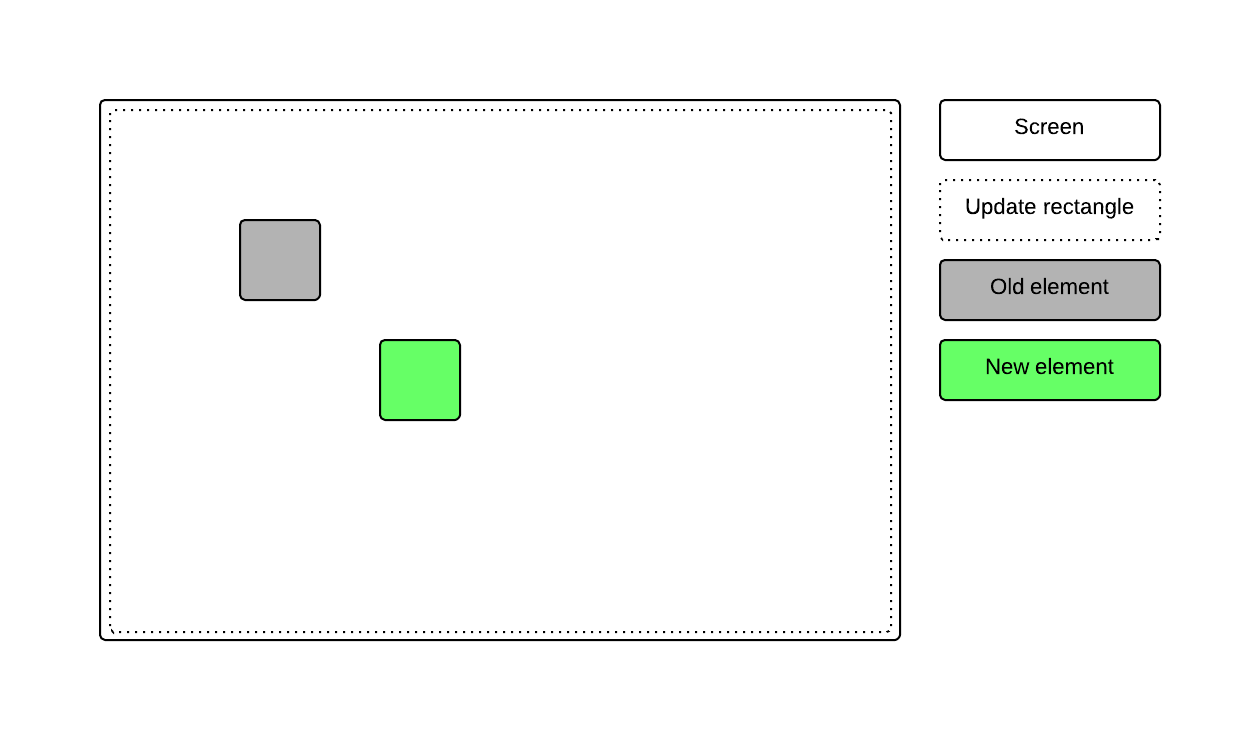
\includegraphics[width=11cm]{img/update_entire_screen.png}\\
	\textbf{Double screen update} \\
	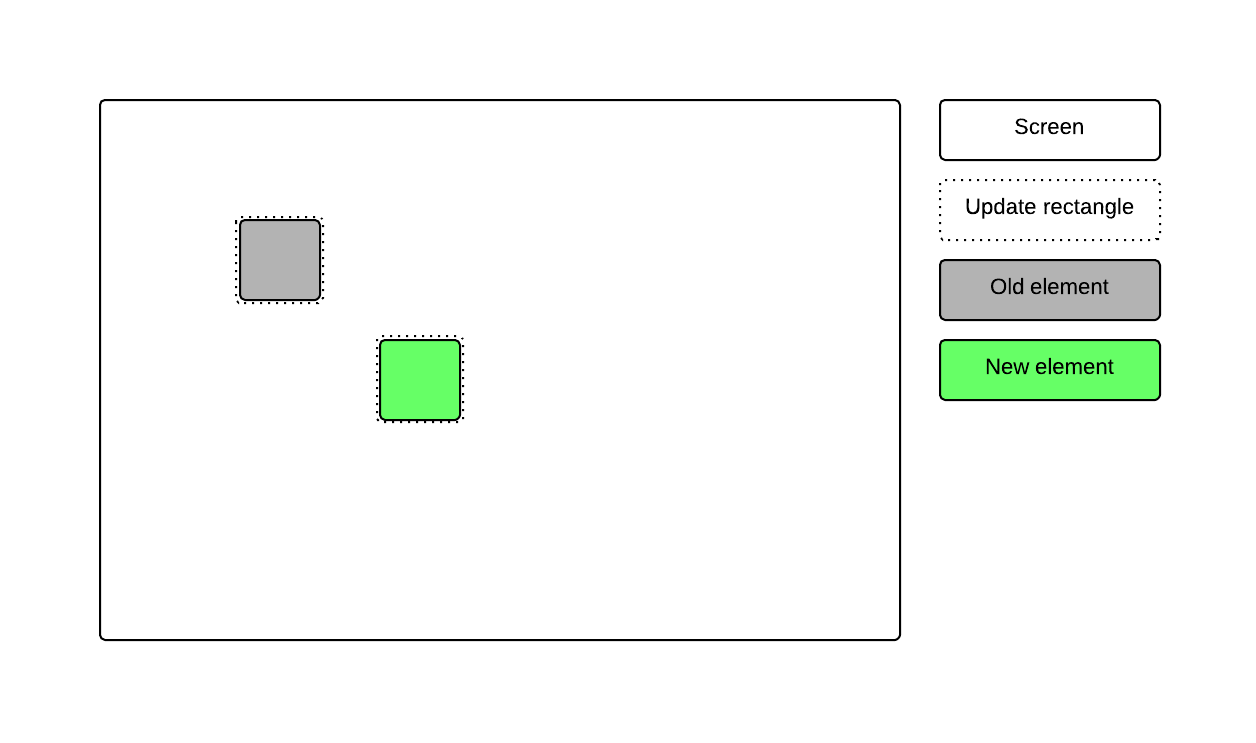
\includegraphics[width=11cm]{img/update_twice.png}\\
	\textbf{Single screen update} \\
	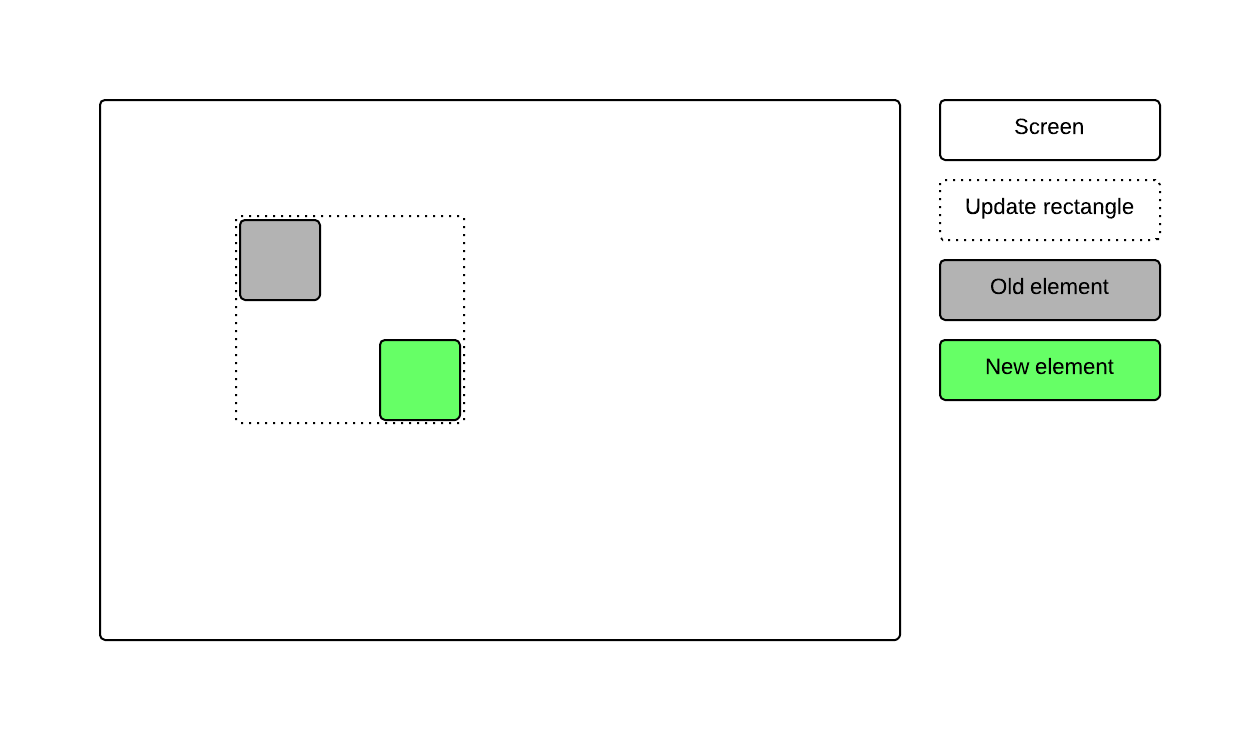
\includegraphics[width=11cm]{img/update_once.png}\\
	\caption{Framebuffer update modes}
\end{figure}

\subsection{Pong}
\label{subsection:pong}
\emph{TODO - Kim}

\subsection{Driver concurrency}
When writing a driver, we need to handle concurrency in the utilization of the driver.
\paragraph{Only on handle allowed}
Using the \vn{device\_open} variable in \mn{driver-gamepad.c}, we made sure that only one handler of the driver could be open at any time. Because the open file operation is protected by a critical region in the Linux kernel, no race conditions can occur setting this variable.\\
\emph{TODO - Finne ut om det er riktig med kritisk region}
\paragraph{Signal mask}
As seen in lines 7-9 of figure \ref{fig:sighandler}, we set a signal mask when assigning signal handlers. By adding signals to this mask, we tell the operating system that these signals should be blocked while the signal handler is running. In this solution, the only code that modifies the game state is signal handlers for \textbf{SIGUSR1} (buttons) and \textbf{SIGALRM} (timer), and by adding these to the signal mask, we guarantee that the signal handlers will run one by one, making it impossible for race conditions and invalid program state.


\subsection{Energy efficiency}
\label{subsection:energy-efficiency}
As we are no longer programming on the "bare metal", we have less control over the software running on the chip. \emph{uClinux} have certain requirements regarding timers and other peripherals, and \cite{compendium} states that "all relevant clocks are already turned on", which we consider as a statement that says the oscilator setup is fixed, and should not be altered for this exercise. Still, we could use some techniques to reduce the energy consumption.

\subsubsection{Interrupts and signals}
We implemented our driver so no polling mechanisms were needed (as described in section \ref{subsection:signals-and-interrupts}). As a consequence, the program will stay most of its time in a \emph{pause()} loop, leaving the CPU and IO buses free to do other stuff (or  sleep). This behaviour decreases power consumption.

\subsubsection{Optimizing screen update}
As described in section \ref{subsubsection:framebuffer-update-modes}, we try to limit the area of the screen we update. We have been adviced that tuning this area have an impact on performance and energy efficiency.

\subsubsection{Tickless idle}
\begin{figure}[h]
	\centering
	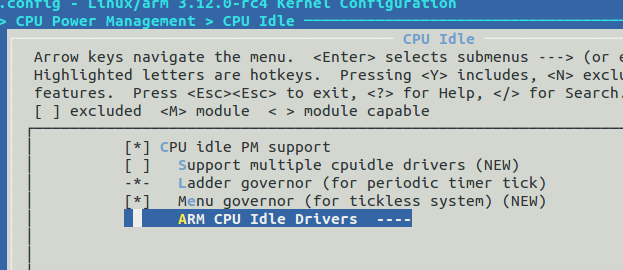
\includegraphics[width=12cm]{img/tickless.png}
	\caption{Configuring the kernel to tickless idle}
	\label{fig:tickless}
\end{figure}
Because our game is handeled entirely by signal handlers, leaving the main program in a pause loop, we wanted to reduce the power consumption while waiting for an interrupt/signal. In order to do that, we were adviced to put the kernel in a mode known as tickless idle. This turns off the normal periodic timer interrupts, which decreases power usage.\\
\\
Tickles idle was enabled in the \emph{kernelconfig} by setting \emph{Idle dynticks system (tickless idle)} in \emph{General setup $\rightarrow$ Timer subsystem $\rightarrow$ Timer tick handling} (see figure \ref{fig:tickless}). This sets the \emph{NO\_HZ\_IDLE} flag.


\newpage \section{Results and Tests}


\subsection{uClinux}
After building and flashing \emph{uClinux} on the chip, we verified that we had a working Linux distribution by connecting to its shell with \emph{miniterm.py} and running Linux commands like \emph{ls} and \emph{cat}. In addition to this, we saw Tux on the screen, indicating that \emph{uClinux} was properly installed.

\subsection{Gamepad driver}
\begin{figure}[h]
	\centering
	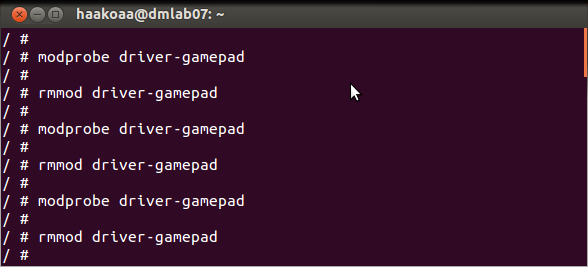
\includegraphics[width=12cm]{img/modprobe.png}
	\caption{Adding and removing the module several times}
	\label{fig:modprobe}
\end{figure}
Testing that the gamepad driver delivers the correct data to the user space is left to our game. If the game functions as expected, we can therefore conclude that the gamepad driver reads and delivers the correct data. Please read on (section \ref{subsection:pong-testing}) to verify the correctness of this.\\
\\
In addition to delivering the correct data on time, it is really important that the driver cleans up properly by deallocating and freeing various data structures used for it's operation. Failing to do so, might cause memory leaks in kernel space; a situation where memory does not get freed before system reboot. Besides from being very accurate (making sure each allocation call had a corresponding deallocation call) in writing the drivers probe and close functions, we tested that we were able to load and uload our kernel module multiple times. We did a test by calling \emph{modprobe driver-gamepad} and \emph{rmmod driver-gamepad} consecutively three times, checking that neither of the calls yielded any error messages. As we can see in figure \ref{fig:modprobe}, the test was a success.

\subsection{Pong}
\label{subsection:pong-testing}
When designing a game, user experience is everything, and it is important that the system behaves as expected. In particular, we focused on the following aspects:

\paragraph{Game behaviour}
The game should follow the rusles of pong. In particular:
\begin{itemize}
	\item The ball should bounce off the player paddles, in addition to the upper and lower walls.
	\item If a player miss the ball, the game should reset.
	\item Up and down buttons on each controller should control the corresponding player paddle. The paddle should move as long the button is pressed down, within it's legal horizontal bounds.
\end{itemize}

\paragraph{Performance}
The game speed should never reduce and the frame update rate should stay at 24 FPS. No player interaction should exhaust the computation resources of the chip, making the game slower.  

\paragraph{No rendering artifacts}
No artifacts with the elements drawn on the screen should appear. By that, we mean that all rectangular shapes should stay in the same color and shape during the game. An example of unwanted behaviour is shown in figure \ref{fig:pong_overlapping}, where the ball removes some pixels from the paddle. In addition to this, no flickering of any screen elements should be present. \\
\\
The game behaviour was tested by playing the game over and over (the game is actually quite entertaining) looking for unexpected behaviour. We confirmed that the game behaved as expected, with one minor flaw: The player movement has unintuitive behaviour if two buttons are pressed at the same time. If up is pressed while down is already pressed, the paddle will move up, but when up is released again, the paddle will stop moving. The most intuitive behaviour would be to let the paddle move down, as the down button is pressed. We decided to not fix this issue, because it requires extra book-keeping in the application. The solutioun is simple: Don't press up and down at the same time.\\
\\
Testing performance and rendering has very much to do with the next section, where we will elaborate on different rendering modes.

\subsection{Energy efficiency and performance}

\subsubsection{Performance and energy efficiency with different frame update modes}

\subsubsection{Tickless idle}

\subsection{Further development}
\paragraph{Memory Mapping}
Memory mapping is a technique used to transfer data between kernel space and userspace without copying. It is the fastest way to handle larger amount of data. The screen module uses this technique when writing to the framebuffer. We thought our driver could benefit from offering a way to use mmap to read the values of the buttons pressed. We attempted to create open and close functions for mmap and assign them to their respective fields in the \emph{vm\_operations} struct. Also a \emph{fault} function where created, wich seems to be the inheritor after the \emph{nopage} got removed. Lastly a function to assign the file data to the virtual memory data where created and assigned to the \emph{mmap} field of the \emph{file\_operations} struct. We failed however to get this to work (, wich is why it is described here and not in the \emph{description of methology} section). It seemed like the \emph{mmap} fuction never got called. Benjamin, who also thought it would be nice of our driver to support memory mapping, where helpfull but unsucessfull when trying to find the problem with us. He did however come with some suggestions where to look for clues, such as in the source code of the framebuffer. As it was not part of the assignment, and since we felt that it had allready taken to much of our time, we did not proceed with any further investigations at this point.


\newpage \section{Evaluation of Assignment}


\newpage \section{Conclusion}
Even tough we already had some experience with C programming from the Compilers course, this exercise has made us grow as C programmers. We found the GPIO control to be more or less the exact same as in the previous exercise. The only difference was the language used. The same goes for the interrupt handling. The DAC however, was something neither of us had experience with. Feeding the DAC with data was easy. However, controlling the sound, having multiple tracks playing over each other and creating music required a lot of thinking. Having tested the different types of soundwaves, we learned that the triangle shape gave the smoothest sound but also the lowest. \\

We also feel that our application is energy efficient, taking into account that we are using the CPU to feed the DAC. Since we are using a low energy timer we are only using half the amperage when playing sounds, and when idle we are saving a great amount of energy as the system is in deep sleep. Even though we did not use the DMA, we feel sucessful in lowering the energy consumption of the system.
   


\newpage \section{Aknowledgements}
As always, we could like to thank our student assistant, \emph{Benjamin Bjørnseth}, for assisting us at the lab hours. In addition to helping us with both technical and non-technical questions, Benjamin contributed in stimulating suggestions and encouragement.\\
\\
In addition to Benjamin, we would also like to thank our lecturer \emph{Asbjørn Djupdal} for guidance regarding configuring the Linux kernel to run with tickless idle.


\newpage \section{References}
\lipsum[3-5]


\end{document}
